\chapter{Theory}
The purpose of this chapter is to give a brief overview of the key theories that have informed my decision during the course
of this project. Though the project has been mainly empirical through numerical studies and implementation, the theory provides 
invaluable insights for the design process and interpretation of results. First, I will discuss some theory of thin-film solar cells, leading to the design choices of my datset generation.
First, I will discuss Fabry-Perot interferometers, as these share many optical properties with thin film-solar cells.
I will then briefly introduce the theory behind rigorous coupled wave analysis (RCWA), which has been the workhorse of the generated data in this project. 
Since I have compared my results with the commercial finite-element method solver COMSOL, I will briefly introduce finite element method as well. 
I will discuss the adjoint method, reverse mode differentiation of electromagnetic problems, and the outlook on surrogate models for optimization.

\label{sec:theory}
% Introduction to methods chosen here.
\section{Thin-Film Solar Cells}
As discussed in section \ref{sec:thinfilmintro}, due to the prevalence of crystalline silicon in the global photovoltaic market and litterature, I will in this project focus on crytalline silicon as the active material of the solar cells, though to note, 
the employed methods would also work with other active materials. 

\begin{figure}[htbp]
    \centering
    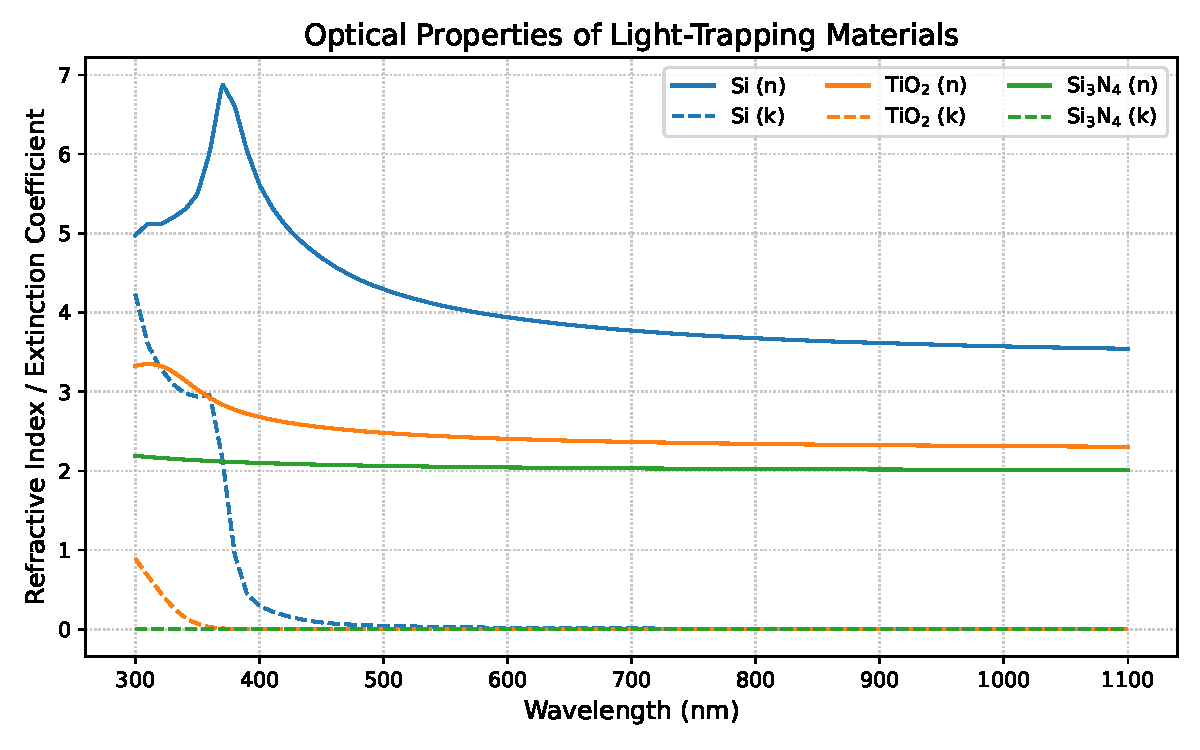
\includegraphics[width=0.8\textwidth]{figures/refractive_indices.pdf}
    \caption{Refractive index (n, solid) and extinction coefficient (k, dashed) profiles of Crystalline Silicon (Si), Titanium Dioxide (TiO$_2$), and Silicon Nitride (Si$_3$N$_4$) across the visible and near-infrared spectrum. Silicon is seen to consistently have the highest refractive index, but also has the highest exctinction coefficient leading to potential parasitic losses in the grating.
    Silicon Nitride is nearly lossless across the entire region, and has an almost constant refractive index near 2.}
    \label{fig:refractive_indices}
\end{figure}

To query the performance of gratings of multiple different materials, I have chosen to include in my study three high-refractive index materials.
First, as a baseline, the gratings are explored in the material of crystalline silicon. Having a high refractive index in much of the solar spectrum might allow trapping light better.
I then explore the two, low loss and medium high refractive index materials of TiO$_2$ and Si$_3$N$_4$. More materials could be included without changing the employed methods.
As previosly mentioned, high refractive index methods are preferred because of the so called Yablonovitch limit, that says that the optical path length of an active material can be increased by a factor $~4n^2$, where n is the refractive inddex.
Having low extinction coefficient $k$, i.e. the imaginary part of the refractive index, also reduces parasitic loss of energy in the grating layer itself. Figure \ref{fig:refractive_indices} shows the refractive index and exctinction coefficients of the chosen materials.

The optical performance of light trapping layers differs based on the polarization of light. Sunlight is essentially unpolarized. The total incoming field is given by
\begin{equation}
\label{eq:unpolarized}
\mathbf{E}_{total} = \mathbf{E}_p + \mathbf{E}_s,
\end{equation}
where $\mathbf{E}_p,\mathbf{E}_s$ is p-polarized s-polarized incoming light respectively. As aborptance is proportional to the intensity, it is seen
that the time average of the intensity of the field is given by
\begin{equation}
\label{eq:average}
\left<|\mathbf{E}_{total}|^2\right> = \langle |\mathbf{E}_{p}|^2 \rangle + \langle |\mathbf{E}_{s}|^2 \rangle + 2\langle \mathbf{E}_{p} \cdot \mathbf{E}_{s} \rangle = \langle |\mathbf{E}_{p}|^2 \rangle + \langle |\mathbf{E}_{s}|^2 \rangle,
\end{equation}
where it has been used that the two fields are orthogonal to each other. Even if a time harmonic term projected the two fields onto a common axis, the rapidly oscillating phase difference would average out to zero.
because of this reason, and as a choice going forward, all quantities will be found for both p-polarization and s-polarization. Final performance might then be averaged over both polarizations in the end.
The percentage of incoming light power is described by incidence angle of light $\theta$ and the total power density of the incoming light $P_in$.
$P_{projected} = \cos{\theta} P_{in}$.
A figure of interest for solar cells is the so-called short circuit current, given by the expression
\begin{equation}
\label{eq:shortcircuitcurrent}
J_{sc} = \frac{q}{hc}\int_{\lambda_{min}}^{\lambda_{max}}\lambda A(\lambda)I_{AM1.5g}(\lambda) d\lambda,
\end{equation}
where $q$ is the elementary charge, $h$ is the planck constant, $c$ is the speed of light, $\lambda$ is the free space wavelength of incoming light, $I_{AM1.5g}$ is the standard reference of incoming intensity of sunlight, which scales with incident angle on the solar sell, and 
$A(\lambda)$ which is the dimensionless absorptance of wavelength $\lambda$. The entire short circuit current may be derived as follows. The number of photons present in the irradiating sunlight is given by
$$
\text{Number of photons} = \text{Incoming Power} / \text{Power per Photon} = I_{AM1.5g} \cdot \left(\frac{hc}{\lambda}\right)^{-1}
$$
If perfect quantum efficiency is assumed, and every photon absorbed excites exactly one charge carrier electron, the reward current for every electron is $q$. This means the short circuit current is then
$$
J_{sc}(\lambda) = q \cdot \text{Number of photons} \cdot A(\lambda) = \lambda A(\lambda) I_{AM1.5g}(\lambda) \frac{q}{hc}.
$$
This is the generated current for every single wavelength, so the total current integrates over $\lambda$, and equation \ref{eq:shortcircuitcurrent} is obtained.
The absorptance is given by
\begin{equation}
\label{eq:absorptance}
A(\lambda) = \frac{P_{abs}(\lambda)}{P_{in}} = \frac{1-R(\lambda)-T(\lambda)}{P_{in}},
\end{equation} 
the absorptance is a dimensionless quantity. For solar tracker farms, the solar cells are angled to always aim the incoming sunlight to hit the solar cells at normal incidence. As such, for
solar tracker farms, the maximum absorptance at normal incidence is desired.
For stationary solar cells, such as solar cells installed on the roofes of houses, the best absorptance over a range of incidence angles is desired.
I've chosen to focus primarily on normal incidence, though the dataset I've generated includes randomly sampled incidence angles for all structures, as well as normal incidence.

The Short circuit current is easily obtained after the fact, so going forward, I will be focusing on calculating the dimensionless $A(\lambda)$ in the film layer.

\section{Fabry-Perot Interferometers}
Though the proposed structures, consisting of a backreflector either assumed to be silver (Ag) or an ideal material with near perfect reflectance, a film of crystalline silicon of height $1000-3000$ nm, and a grating layer,
are not exactly Fabry-Perot Interferometers, they do share many similarities. A pure Fabry-Perot interferometer is an optical cavity made of two parallel reflecting surfaces. Like in a microwave, if reflecting bounces of light inside the cavity 

\begin{figure}[htbp]
    \centering
    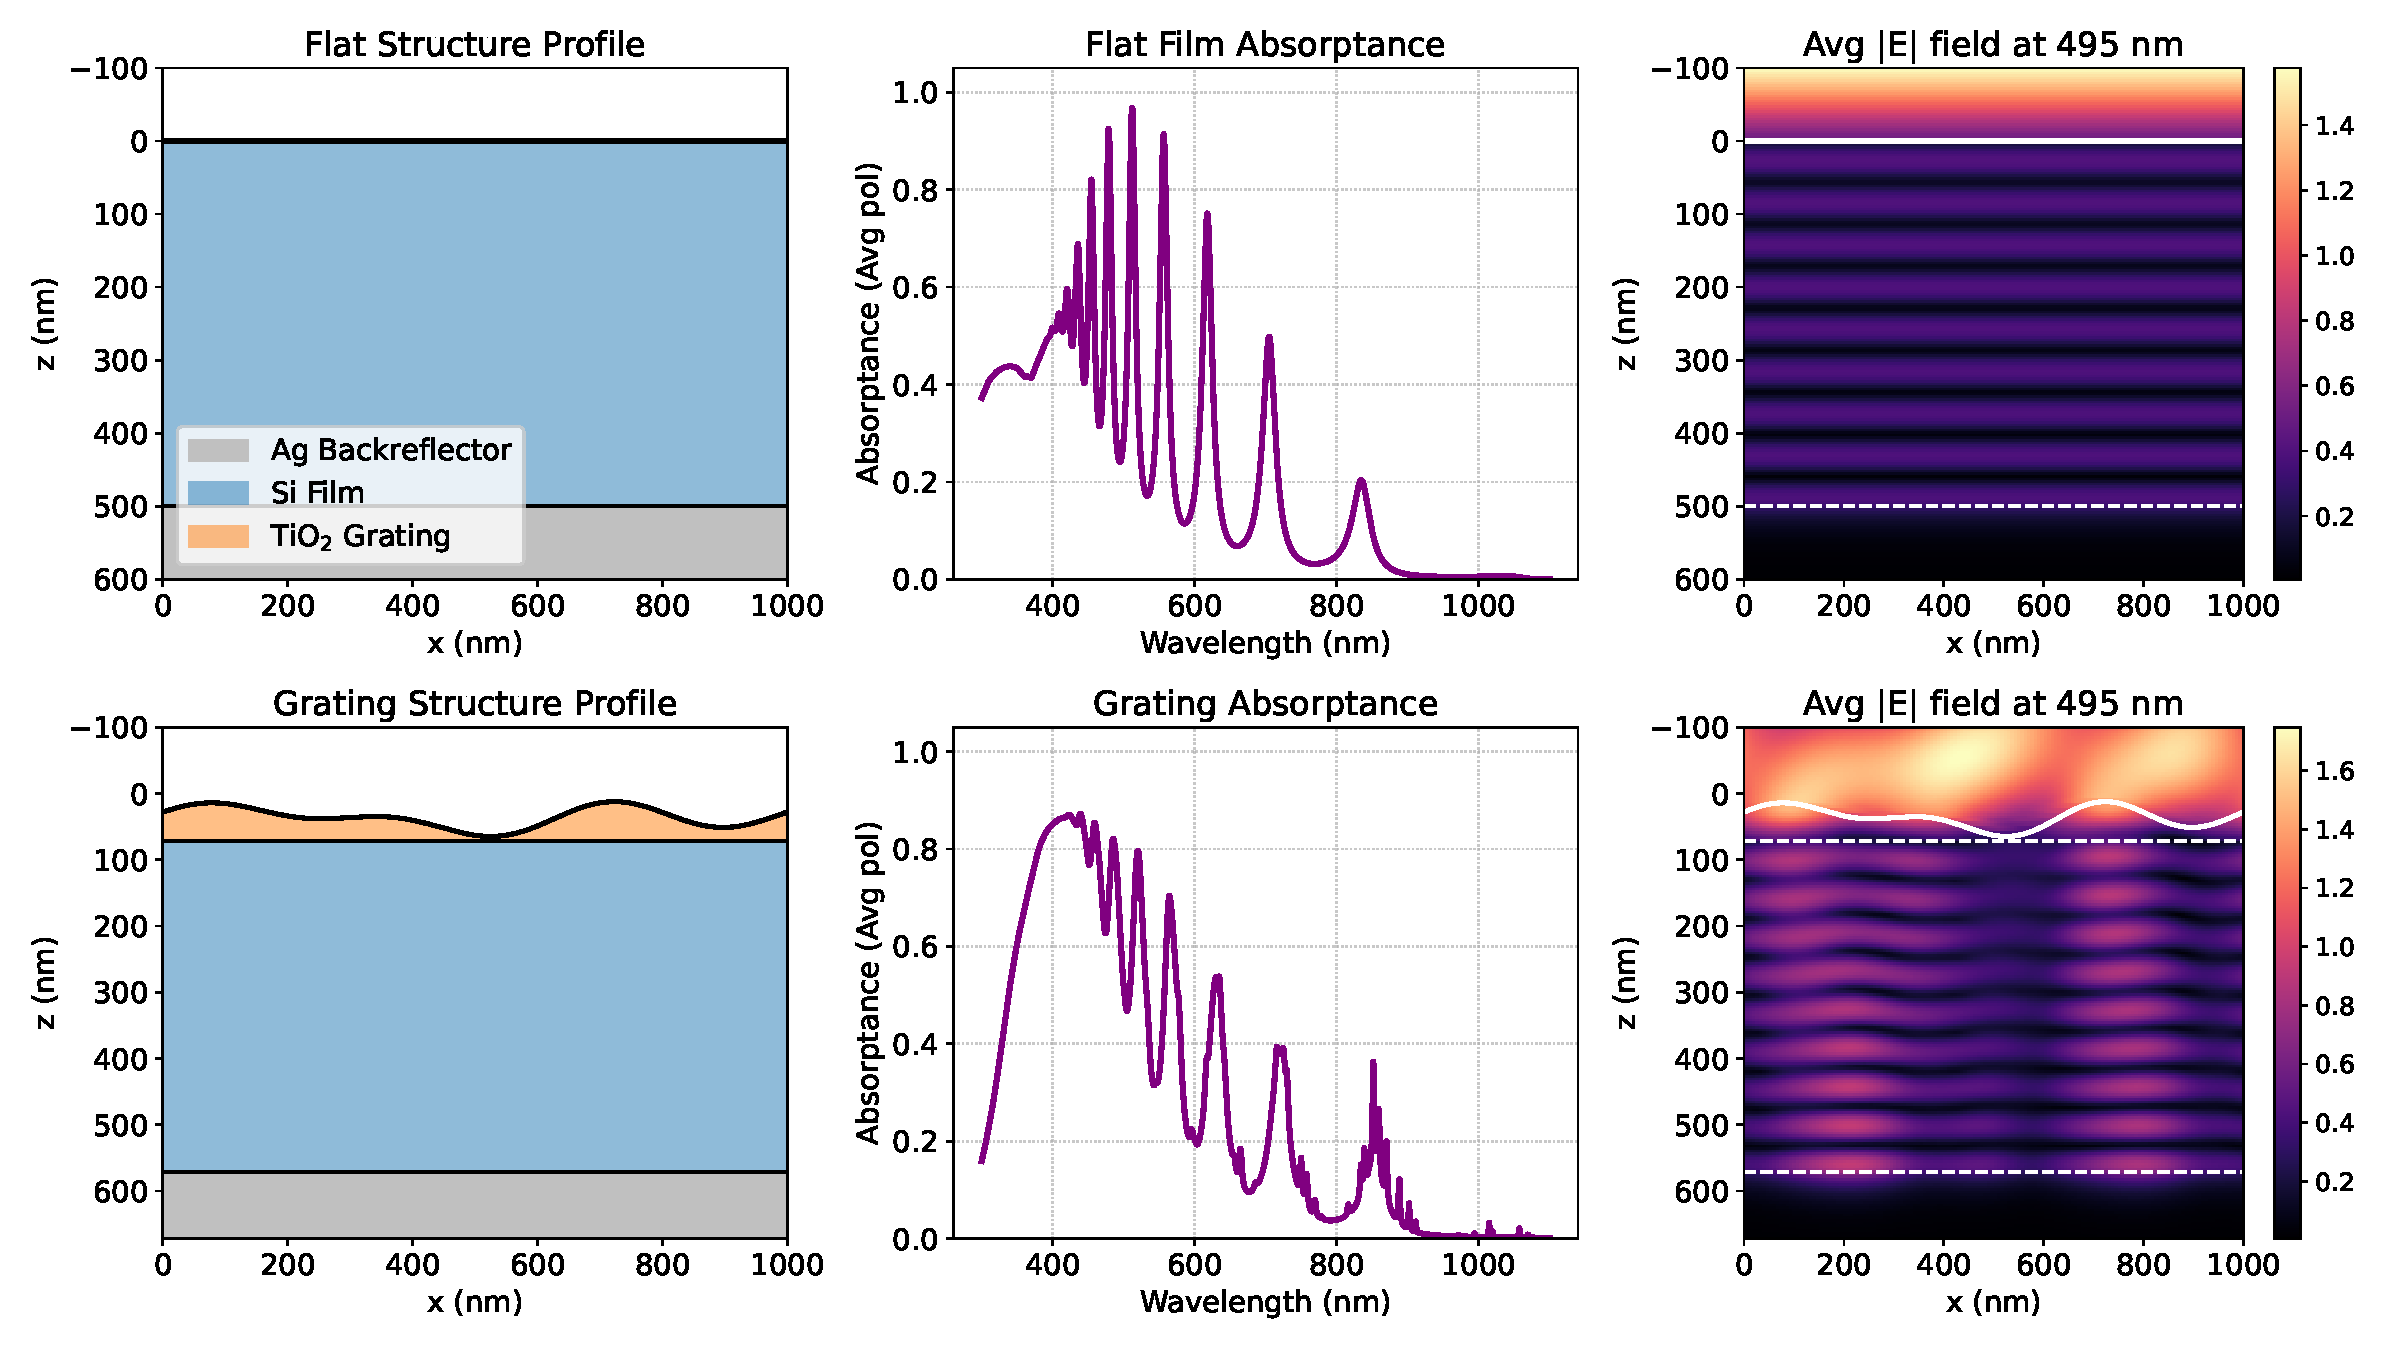
\includegraphics[width=0.95\textwidth]{figures/fabry_perot_grid.pdf}
    \caption{Interferometer effects in a bare flat film (top) versus a patterned grating structure (bottom). The left column presents the xz-plane structure profile (TiO$_2$ grating on Si film with an Ag backreflector). The middle column shows the polarization-averaged absorptance spectrum at $\theta = 30^\circ$. The right column displays the polarization-averaged electric field magnitude $|E|$ at $\lambda = 495$ nm.
    Notice that the smooth part of the curve lasts for longs and more small resonance peaks appear at the fourier grating. However, the overall shape remains much the same. }
    \label{fig:fabry_perot}
\end{figure}
Without going too much into detail, a key result of fabry-perot interferometers in wavelength space is that
peak transmittance (or equally, absorptance if the material is lossy) occurs when constructive interference of backward and forward scattered light occurs. It can be shown\footnote{\url{https://en.wikipedia.org/wiki/Fabry-Perot_interferometer}} that the wavelength seperation between 
adjacent transmission (Absorptance) peaks is given by
\begin{equation}
\label{eq:fabry perot}
\Delta \lambda \approx \frac{\lambda_0^2}{2n_g h\cos{\theta}},
\end{equation}
where $\lambda_0$ is the wavelength of the nearest peak and $n_g$ is the refractive index of the crystalline silicon film. Noteably, the lower the wavelength, the more densely spaced the absorptance peaks will be.
for a film height of 3000 nm, the peaks at the lower wavelengths of $\lambda_0\approx 400 \text{nm}$, the spacing between peaks is $\Delta\lambda \approx5.49 \text{nm}$. This implicitly sets a limit on how rough the wavelength sampling can be in the dataset generation.

figure \ref{fig:fabry_perot} show the structure profile, absorptance curve from $300 \text{nm}$ to $1100$ nm and average field at a wavelength of $495$ nm of a Fabry-Perot like resonator, and the bottom row shows almost the same structure, but it has a fourier patterned grating of TiO$_2$.
One thing to note is that the location of the absorptance peaks approximately overlap. Non of them are meaningfully widened, but for about $800$ nm, the spectrum starts to exhibit smaller peak oscillations. If the wavelength resolution were even higher, perhaps these peaks would have noticeable heights.
the interpretation is of course that the grating can kick the momentum of the incoming light into a nearby resonance. Another thing to note is that the region without oscillations is significantly widened. This is the region where crystalline silicon film absorbs/reflects light well enough, forward and backward reflections cant live in the film.
The light is either absorbed before standing waves occur with their high frequency oscillations, or the light is reflected. But for light of about 400 nm, the absorptance is for the given grating higher than $80\%$, indicating that the graing works well as an anti-reflective coating (ARC) here.

\section{Rigorous Coupled Wave Analysis}
\label{classical_solvers}
This subsection will introduce the concept of RCWA, a method in numerical photonics suited well
for stacked periodic structures in the x and y axis with a period $\Lambda_x,\Lambda_y$ respectively, and where each layer is homogeneous in the z-direction\cite{torcwa}.
The structure's optical properties are completely described by the relative permitivity $\epsilon$ and relative permeability $\mu$ of each layer, meaning that each structure
will have a geometry described by
\begin{equation}
\label{eq:permittivity_periodicity}
\epsilon(x,y,z)_N = \epsilon(x + m \cdot \Lambda_x, y + n \cdot \Lambda_y)_N, m,n \in \mathbb{Z}
\end{equation}
and 
\begin{equation}
\label{eq:permeability_periodicity}
\mu(x,y,z)_N = \mu(x + m \cdot \Lambda_x, y + n \cdot \Lambda_y)_N, m,n \in \mathbb{Z},
\end{equation}
where $m$ and $n$ are integers and the subscript $N$ denotes the $N$'th layer of the structure. For the entirety of this project, the designed
fourier patterned light trapping layers will be designed using crystalline silicon ($Si$), Titanium Dioxide ($TiO_2$) and Silicon Nitride ($Si_3N_4$), which
are all nonmagnetic, so the relative permeability $\mu = 1$. In general, $\epsilon$ and $\mu$ will be $3 \times 3$ tensors, but for isotropic and linear materials these are scalars.
The equations solved for are of course the Maxwell equations, namely Faraday's law
\begin{equation}
\label{eq:faraday}
\nabla \times \mathbf{E} = -\mu_0\mu(x,y)\frac{\partial\mathbf{H}}{\partial t}
\end{equation}
and Ampere's law
\begin{equation}
\label{eq:ampere}
\nabla \times \mathbf{H} = \epsilon_0\epsilon(x,y)\frac{\partial\mathbf{E}}{\partial t},
\end{equation}
Where $\epsilon_0$ and $\mu_0$ are the vacuum permitivity and vacuum permeability respectively. The structures are assumed free of charge and current,
$$
\nabla \cdot (\epsilon \mathbf{E}) = 0
$$
and
$$
\nabla \cdot (\mu \mathbf{H}) = 0.
$$
At a single frequency and in homogeneous media, the eigenmodes of Maxwell's equations are solved by plane waves, see \cite{griffiths} section 9.2.1 for example,
meaning
\begin{equation}
\label{eq:planewaveE}
\mathbf{E} = \mathbf{E}_0 \exp{i(\mathbf{k}\cdot\mathbf{r} - \omega t)}
\end{equation}
and
\begin{equation}
\label{eq:planewaveH}
\mathbf{H} = \mathbf{H}_0 \exp{i(\mathbf{k}\cdot\mathbf{r} - \omega t)},
\end{equation}
Where $\mathbf{E}_0$ and $\mathbf{H}_0$ are the (complex) amplitudes of the fields, with the physical fields being the real parts of
$\mathbf{E}$ and $\mathbf{H}$, $\mathbf{k}$ being the wavevector, i.e. the spatial frequency, and $\omega$ being the frequency of the fields, also given by the dispersion relation
$\omega = \frac{c|\mathbf{k}|}{n(\lambda)}$, where $\lambda$ is the wavelength of the light.
It is noted that conservation of momentum leads to the spatial components of the wavevector only having two dgrees of freedom, i.e.
\begin{equation}
\label{eq:dispersionk}
|\mathbf{k}| = \frac{2\pi n(\lambda)}{\lambda} = \sqrt{k_x^2+k_y^2+k_z^2} = k_0,
\end{equation}
and in general, for an incident angle $\theta$ and azimuthal angle $\phi$, the x and y components will be chosen by
\begin{equation}
\label{eq:inc_ang_k}
(k_x,k_y) = k_0(\sin{\theta}\cos{\phi},\sin{\theta}\sin{\phi}).
\end{equation}

Inserting equations \ref{eq:planewaveE} and \ref{eq:planewaveH} in equations \ref{eq:faraday} and \ref{eq:ampere} converts the time derivative to
an algebraic factor of $-i\omega t$, meaning that the equations appear in their time harmonic form, common to many frequency domain numerical methods in photonics,
\begin{equation}
\label{eq:THfaraday}
\nabla \times \mathbf{E} = i\omega\mu_0\mu(x,y)\mathbf{H}
\end{equation}
\begin{equation}
\label{eq:THampere}
\nabla \times \mathbf{H} = -i\omega\epsilon_0\epsilon(x,y)\mathbf{E}.
\end{equation}



Owing to the periodicity of the system, see equations \ref{eq:permittivity_periodicity} and  \ref{eq:permeability_periodicity}, both the electromagnetic fields and the permitivity and permeability may
be written as their truncated fourier series in the x- and y-directions as below. Truncating the electromagnetic fields to order $M,N$ in $x,y$ makes RCWA a semi-analytical method
precise only to this fourier order. The final fields are reconstructed as an inverse Fast Fourier Transform, so including enough fourier orders is an important convergence criterion.
\begin{equation}
\label{eq:fourierPermitivity}
\epsilon(x,y) = \sum_{m=-2M}^{2M}\sum_{n=-2N}^{2N}\epsilon_{m,n}\exp{i(mL_xx+nL_yy)},
\end{equation}
\begin{equation}
\label{eq:fourierPermeability}
\mu(x,y) = \sum_{m=-2M}^{2M}\sum_{n=-2N}^{2N}\mu_{m,n}\exp{i(mL_xx+nL_yy)},
\end{equation}
\begin{equation}
\label{eq:fourierFaraday}
\mathbf{E} = \exp{i\mathbf{k}\cdot\mathbf{r}}\sum_{m=-M}^{M}\sum_{n=-N}^{N}\mathbf{E}_{m,n}\exp{i(mL_xx+nL_yy)},
\end{equation}
\begin{equation}
\label{eq:fourierAmpere}
\mathbf{H} = \exp{i\mathbf{k}\cdot\mathbf{r}}\sum_{m=-M}^{M}\sum_{n=-N}^{N}\mathbf{H}_{m,n}\exp{i(mL_xx+nL_yy)},
\end{equation}
where $L_x = \frac{2\pi}{\Lambda_x}$ and $L_y = \frac{2\pi}{\Lambda_y}$, 
and the parameters $\epsilon_{m,n}, \mu_{m,n}, \mathbf{E}_{m,n}$ and $\mathbf{H}_{m,n}$ are the fourier amplitudes of the $m,n$'th diffraction order.
It is worth mentioning, that since the momentum of light is always conserved, $k_z$ implicitly depends on the expansion orders $m,n$, and writing out the k-vector in full, including the fourier components, yields
\begin{align}
\label{eq:kmn}
\mathbf{k}_{m,n} &= (k_x+mL_x,k_y+mL_y,k_z(m,n)) = \\ &= \left(k_x+mL_x,k_y+mL_y,\sqrt{k_0^2-(k_x+mL_x)^2-(k_y+mL_y)^2}\right),
\end{align}
where equation \ref{eq:dispersionk} has been used. The physical interpretation of the fourier series of the electromagnetic fields is then made obvious;
the different terms are different diffraction orders, each with part of the initial z-component momentum kicked into either the x- or y-direction.
It is noted how the permitivity and permeability is expanded to twice the order of the electromagnetic fields $E$ and $H$. This arises
from the fact that the algebraic components of equations \ref{eq:faraday} and \ref{eq:ampere} include products of Fourier series, so to reach order $M,N$ in the electromagnetic fields,
the permitivity and permeability must be truncated at twice the order. An example for just one fourier order will be given below, but for more details, I refer to \cite{fmm}.
By inserting 



% Detail the rigorous coupled-wave analysis (Torcwa)

\section{Finite Element Method}


\section{The Adjoint Method}
\label{sec:adjoint}
Nanophotonic topology optimization leverages computational optimization  techniques to discover nonintuitive, compact devices, with a high performance
on a clearly defined figure-of-merit. As described by \cite{Hughes2018}. Inverse design starts with the figure of merit,
\begin{equation}
\label{eq:FoM}
\mathcal{L}=\mathcal{L}(x,p),
\end{equation}
and the governing equations in their general form
\begin{equation}
\label{eq:constrainAdjoint}
f(x,p) = 0,
\end{equation}
where x is the state variable, lets say here representing the
electromagnetic fields, whereby $f(x,p)$ represents Maxwell's equations. The  $p$ is the set of real-valued design variables. In this project, this set of design variables will be the set of $a_n,a_m,\phi_n,\phi_m$, along with the film height $h$. You could also see the incident angle $\theta$ and azimuthal angle $\phi_a$ of incoming light 
along with the grating periods $\Lambda_x,\Lambda_y$ as design variables, but for the most case, I have held these constant.
The adjoint method is a method for finding the derivative of the figure of merit with respect to the design variables, where you only need to solve the system forward, for the solution and backward to find an adjoint variable.
Taking first the total derivative with respect to the design variables and using the chain rule, we get
\begin{equation}
\label{eq:totalDeriv}
\frac{d\mathcal{L}}{d p} = \frac{\partial\mathcal{L}}{\partial p} + \frac{\partial\mathcal{L}}{\partial x}\frac{\partial x}{\partial p}.
\end{equation}
The notation here is general by design, and usually both p and x are large vector spaces, so the derivative $\frac{\partial x}{\partial p}$ is a large Jacobian matrix.
In the continuous case, we may get around this by introducing a bright idea and a lagrangian multiplier $\lambda^T$. Utilizing the fact that the governing equation is zero, by the chain rule it must also be true that
\begin{equation}
\label{eq:chainrulegovern}
\lambda^T\frac{dg}{dp} = \lambda^T\frac{\partial g }{\partial x}\frac{\partial x }{\partial p} + \frac{\partial g}{\partial p} = 0
\end{equation}
As this expression is zero, we can freely add it to equation \ref{eq:totalDeriv}. After grouping common terms, we obtain
\begin{equation}
\label{eq:lagrangian}
\frac{d\mathcal{L}}{dp} = \frac{\partial \mathcal{L}}{\partial p} + \lambda^T \frac{\partial f}{\partial p} + \left( \frac{\partial \mathcal{L}}{\partial x} + \lambda^T \frac{\partial f}{\partial x} \right) \frac{\partial x}{\partial p}
\end{equation}
Since $\lambda$ is free, we can choose a vector that kills off the large Jacobian $\lambda^T\frac{\partial f}{\partial x} = -\frac{\partial \mathcal{L}}{\partial x} $,
to get
\begin{equation}
\label{eq:adjoint}
\frac{d\mathcal{L}}{dp} = \frac{\partial \mathcal{L}}{\partial p} + \lambda^T\frac{\partial f}{\partial p}.
\end{equation}
Whereby we have obtained an expression for the figure of merit derived with respect to the set of design variables. \cite{Hughes2018} includes two system variables, the electric field and its conjugate, but the general idea is the same.
Essentially, the original field $x$, which is a forward pass of a physics simulator, has to be solved for, after which the figure of merit dependence is often a scalar derived by a vector value, $\frac{\partial\mathcal{L}}{\partial x}$.
From here, the adjoint field can be simulated backwards by realizing that solving the system for the adjoint variable is essentially the problem in reverse,
$\lambda^T\frac{\partial f}{\partial x} =\frac{\partial f}{\partial x}^T\lambda = -\frac{\partial \mathcal{L} }{\partial x},$ where the intuition is that $f$, that are essentially Maxwell's equations derived with respect to the electromagnetic fields are a the differential operator of Maxwell's  equations, so 
$\lambda$ must be analog to the electromagnetic field in a transverse problem, and the figure of merit derivative $-\frac{\partial \mathcal{L}}{\partial x}$ must be equal to a virtual source. 
Mathematically, this is very close to how gradients flow backwards in reverse-mode auto differentiation software such as Pytorch, and 
by extension TORCWA, \cite{torcwa}. Instead of numerically differentiating the figure of merit by every design variable, the system can be simulated forward, and by trackcing the chain rule, once obtaining the figure of merit, can be efficiently tracked backward.
For an example of the physics, see \cite{Hughes2018}, for more discussion on the adjoint method, see \cite{Hughes2019} and for an example of the reverse mode auto differentiation of for example pytorch, see \cite{torcwa}.

Though this method is powerful, and allows for numerical exact gradients of optical fields with respect to a large number of variables, the optimization problem is still a local optimization problem in a vast design space.
Optimization still requires solving large scale forward problems for every single optimization step. As discussed in the introduction, 